% TODOS
% Does J need to be normalized, wrt Rindler and Minkowski
% Work out details of Green's function
\documentclass[12pt,a4paper]{article}
\usepackage[width=.75\textwidth]{caption}
\usepackage{graphicx}
\usepackage{authblk}
\usepackage{amsmath}
\usepackage{amsfonts}
\usepackage{braket}
\usepackage{epigraph}
%\usepackage{mathrsfs}
\usepackage[mathscr]{euscript}
\usepackage[top=2cm, bottom=2cm, left=2cm, right=2cm]{geometry}
\usepackage{fancyhdr}
\newcommand*\diff{\mathop{}\!\mathrm{d}}
\newcommand\restr[2]{{% we make the whole thing an ordinary symbol
  \left.\kern-\nulldelimiterspace % automatically resize the bar with \right
  #1 % the function
  \vphantom{\big|} % pretend it's a little taller at normal size
  \right|_{#2} % this is the delimiter
  }}
\setlength{\epigraphwidth}{0.8\textwidth}

% \pagestyle{fancy}
\begin{document}

%title and author details
\title{Field Theoretic Thrust of an Accelerating Frame}
\author[1]{Kevin Player\footnote{kplaye@gmail.com}}

\maketitle

\epigraph{The Unruh effect tells us that what we call particles is really just a matter of perspective.}{Lee Smolin}

\abstract{We analyze the quantum field theoretic framework in which Unruh radiation arises, interpreting the radiation as sourced by a driving field. In the Rindler frame, these driving modes span an extended region of time and exhibit a red- and blue-shifted frequency spread due to their support over the full Rindler wedge, resulting in a thermalized response. To refine this picture, we construct an interpolation between these long-lived driving modes and localized wave packets with peaked Fourier spectra that do not display such frequency smearing. This allows us to reinterpret Unruh radiation in terms of thrust—a localized driving effect that excites the field without inducing a thermal response, thereby offering a complementary, nonthermal perspective on acceleration-induced radiation.}

\section{Introduction}
We first present some notation and review the Unruh effect in section 2.  We then introduce a source field in section 3 that exactly captures the particle creation in the cross term of the Bogoliubov transform for Rindler modes extended to Minkowski spave.  In section 4,  we interpolate between the eternal Rindler mode source to a more localized wave packet version, and in section 5 we interpret the results.

\section{Unruh Effect Review and Notation}

We draw notation and standard results from Frodden and Vald{\'{e}}s \cite{Frodden}.

Let $\hbar$ = $c$ = 1. Consider a uniform linear acceleration in $1+1$ dimensional spacetime and use metric signature $\eta = (-1,1)$. The full $1+3$ dimensional case does not add anything to the discussion, so without loss of generality we stick to the dimensions time $t$ and space $x$ where the boost is taking place.  Also, for clarity sake, we stick to the simplest case where $\phi$ is a free massless scalar field.  Even in this simple toy case, we can present our argument.

Consider the free scalar massless Lagrangian
\begin{equation}
\mathscr{L} = -\frac{1}{2} \eta^{\mu\nu}\partial_\mu \phi \partial_\nu \phi.
\end{equation}
We consider positive frequency modes with dispersion relation $\omega_k = |k| > 0$ as solutions to the resulting Klein-Gordon equation 

\begin{equation}
  \Box \phi = -\frac{\partial^2 \phi}{\partial t^2} + \frac{\partial^2 \phi}{\partial x^2} = 0,
 \label{massless-wave-eq}
\end{equation}
where $\Box = \eta^{\mu\nu} \partial_\mu \partial_\nu$. We expand $\phi$ in terms of ladder operators $a_k, a_k^\dagger$

\begin{equation}
  \int \diff k \, a_k \varphi_k(x,t) + h.c.
\end{equation}
where

\begin{equation}
  \varphi(x,t) = \frac{1}{\sqrt{4\pi\omega_k}} e^{i(kx - \omega_k t)}.
\label{amode}
\end{equation}
are positive frequency modes normalized with respect to the Klien-Gordon inner product at any time slice, say $t = 0$,
\begin{equation}
  \left<f, g\right>_{KG} = i \int \diff x (f^* \partial_t g - \partial_t f^* g).
\end{equation}

Consider the $x>|t|$ Rindler ``wedge'' with coordinates
\begin{equation}
  t = \frac{1}{a}e^{a\xi}\sinh{(a\eta)}
\label{sinh}
\end{equation}
\begin{equation}
x = \frac{1}{a}e^{a\xi}\cosh{(a\eta)}
\end{equation}
where $a>0$ is an acceleration parameter (see $I$ in Figure \ref{rindlerw}). These are hyperbolic polar coordinates with an exponential ``radius''.

\begin{figure}[h]
\centering
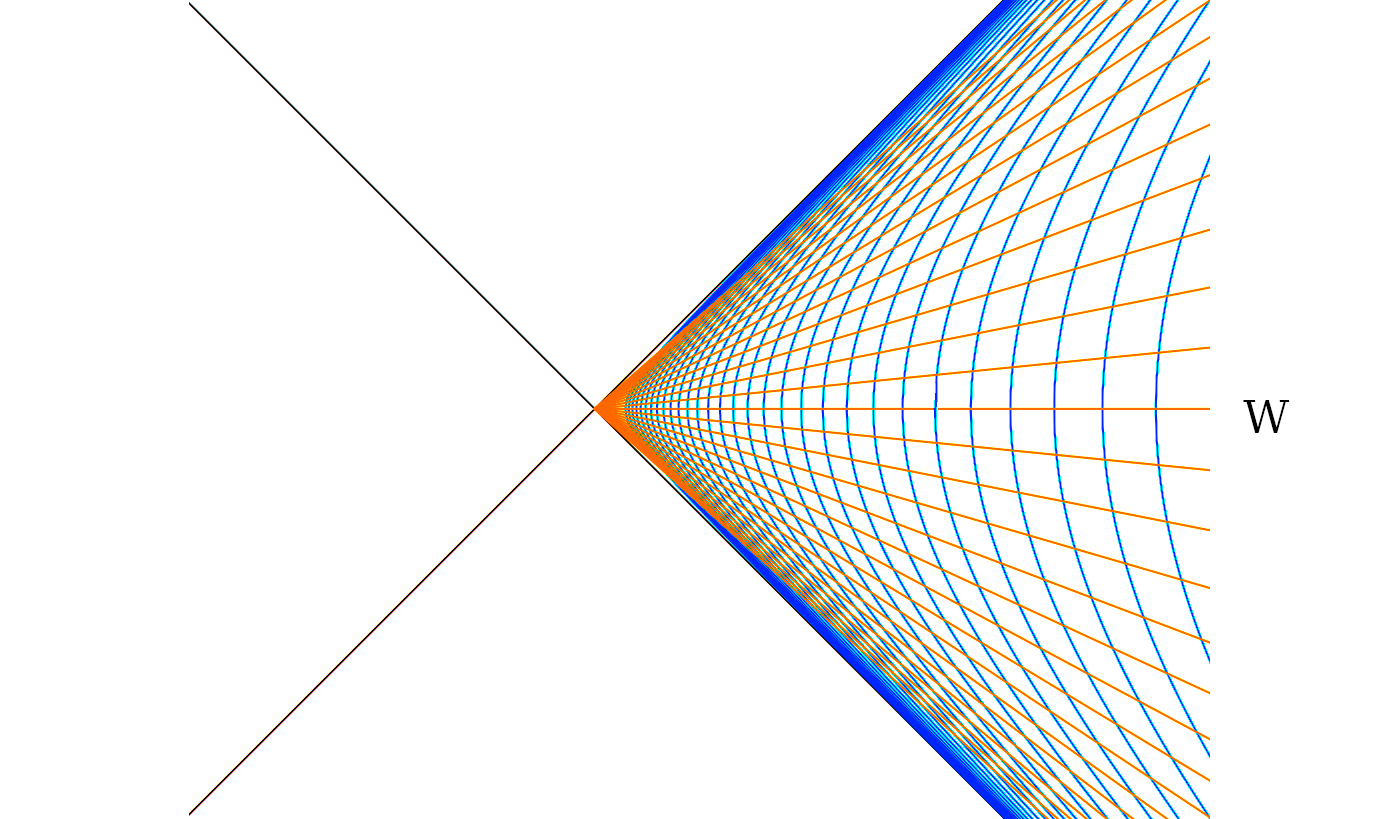
\includegraphics[scale=0.4]{rindler_w.png}
\caption{Rindler wedge $I$ on the right.}
\label{rindlerw}
\end{figure}

The massless Klein-Gordon equation in Rindler coordinates is
\begin{equation}
  \Box \phi = e^{-2a \xi}(-\partial_\eta^2 + \partial_\xi^2) \phi = 0
\end{equation}
which being the same as equation (\ref{massless-wave-eq}) up to a conformal factor, has a basis of solutions with the same form as equation (\ref{amode})
\begin{equation}
 r_k(\eta,\xi) = \frac{1}{\sqrt{4 \pi \omega_k}} e^{-i(\omega_k \eta -k \xi)} + h.c.
\end{equation}
for each wave number $k$ and positive frequency $\omega_k = |k| > 0$.  These ``Rindler modes'' are in terms of $\eta$ and $\xi$ and are thus confined to the Rindler wedge $I$.


Let $u = -t + x$ and $v = -t - x$ be coordinates defined along the light cone.  Each $r_k$ can be extended non-uniquely to the entire $(t,x)$-plane as
\begin{equation}
  \sqrt{4 \pi \omega_k} r_k(x,t) = \left\{\begin{array}{lll}
      g_k^{(1)} h_k^{(1)}(u)&={(au)}^{\frac{i\omega_k}{a}} &=  e^{\frac{i\omega_k}{a} \left(\log(-1) + \log(au)\right)} \text{ for } k>0\\
      g_k^{(2)} h_k^{(2)}(v)&={(av)}^{\frac{i\omega_k}{a}} &= e^{\frac{i\omega_k}{a} \left(\log(-1) + \log(av)\right)} \text{ for } k<0\\  
    \end{array}\right.
\end{equation}
where there is a choice of two branches of the log for each of the two forms of extensions $h_k^{(1)}$ and $h_k^{(2)}$ and the $g_k^{(1)}$ and $g_k^{(2)}$ are normalization factors to be discussed critically shortly. These extensions are functions of $u$ and $v$ respectively, and so are solutions to equation (\ref{massless-wave-eq}). We choose $\log(-1) = -i \pi$ following \cite{Frodden}, and then $h_k^{(1)}$ and $h_k^{(2)}$ are positive frequency modes which once normalized form an alternative basis to the usual $\varphi_k(x,t)$. We then expand
\begin{equation}
  \phi = \int \diff k( c_k^{(1)} h_k^{(1)} + c_k^{(2)} h_k^{(2)}) + h.c.  
\end{equation}
with alternate Minkowski ladder operators $c_k^{(1)}$, $c_k^{(2)}$, $c_k^{(1)\dagger}$, and $c_k^{(2)^\dagger}$. See Figure \ref{analytic} for a picture and summary of these types of modes.
\begin{figure}[h]
  \centering
  \captionsetup{width=0.8\linewidth}
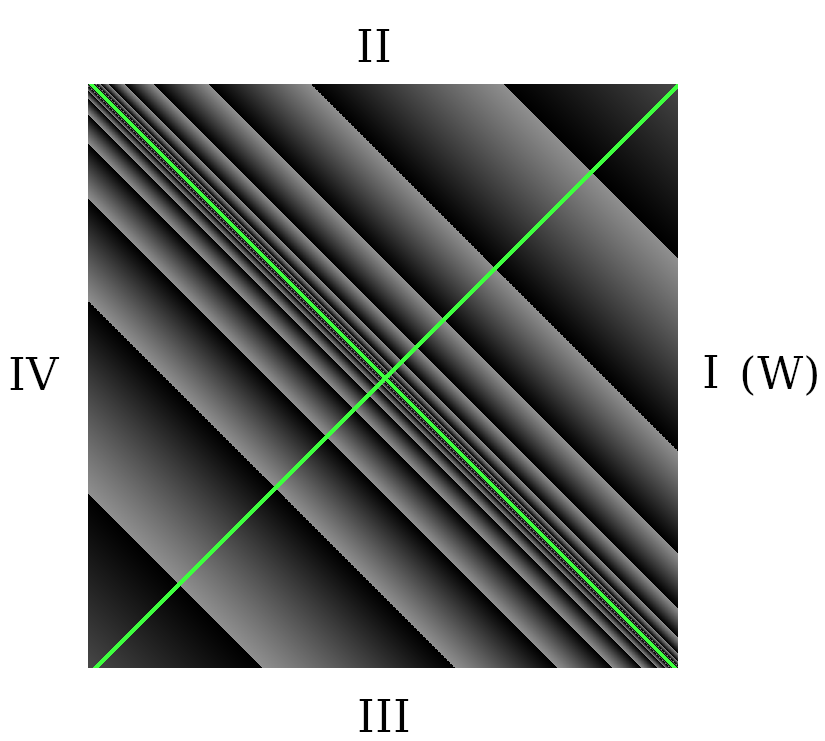
\includegraphics[scale=0.3]{analytic.png}
\caption{The phase of a Rindler mode $r_k$ is shown in gray scale. For $k>0$, $r_k$ is a function of $u$, with a branch of the log at the future horizon of I where $-t + x = u = 0$. $r_k$ is analytically continued around this horizon and can be thought of as an emission from the Rindler observer, blue shifted infinitely into the future in the Minkowski frame. On wedges I and III, $r_k$ is off by a factor of $e^{\pm \frac{\pi \omega_k}{a}}$ in magnitude from wedges II and IV.  A similar situation exists for $k<0$, thought of as absorption by the observer, red shifted from the past horizon, a function of $v$, where I, II vs. III, IV have the $e^{\pm \frac{\pi \omega_k}{a}}$ factor.}
\label{analytic}
\end{figure}

The $\log(-1)$ converts what would otherwise be a pure phase into a exponential factor $e^{\pm \frac{\pi \omega_k}{a}}$.  To be more specific for $k>0$, let $f_k^{(1)} = \restr{g_k^{(1)} h_k^{(1)}}{I}$ and $f_k^{(2)} = \restr{g_k^{(2)} h_k^{(2)}}{IV}$ be the restrictions to the right and left wedges respectively so that $\left|f_k^{(1)}\right| = \left|f_k^{(2)}\right| = 1$ and one can show that
\begin{equation}
  \begin{array}{l}
    \restr{g_k^{(1)} h_k^{(1)}}{I \cup IV} = f_k^{(1)} + e^{- \frac{\pi \omega_k}{a}} f_{-k}^{(2)} \\
    \restr{g_k^{(2)} h_k^{(2)}}{I \cup IV} = f_k^{(2)} + e^{- \frac{\pi \omega_k}{a}} f_{-k}^{(1)}
  \end{array}
\end{equation}

Finally, we turn our attention to the normalization factors $g_k$ and realize the Klien-Gordan dot product on full Minskowsi space as the sum of the dot product on the left and right Rinder wedges.  A negative sign also appears in the sum since $\diff x \rightarrow -\diff x$ from right to left wedges:
\begin{equation}
 \begin{array}{ll}
  \left< r_k, r_k \right>_{KG} &= \left< r_k, r_k \right>_{I} + \left< r_k, r_k \right>_{IV} \\
  &= \left< r_k, r_k \right>_{I} - e^{- \frac{2\pi \omega_k}{a}} \left< r_k, r_k \right>_{I} \\
  &= e^{-\frac{\pi \omega_k}{a}} (2 \sinh \frac{\pi \omega}{a}) \left< r_k, r_k \right>_{I}
  \end{array}
\end{equation}
So $r_k$ is normalized differently on all of $I \cup IV$ than on $I$ and $IV$ seperatly.  This sets $h_k$ as
\begin{equation}
  \begin{array}{ll}
    h_k^{(1)} &= \frac{e^\frac{\pi \omega_k}{2a}}{\sqrt{2 \sinh \frac{\pi \omega_k}{a}}} r_k \text{ for } k>0\\
    h_k^{(2)} &= \frac{e^\frac{\pi \omega_k}{2a}}{\sqrt{2 \sinh \frac{\pi \omega_k}{a}}} r_k \text{ for } k<0\\
  \end{array}
\end{equation}  
This normalization issue is the root cause for Unruh radiation since we pick up a {\bf sinh} factor in the cross term in the Bogoliubov transform
\begin{equation}
  b_k = \frac{1}{\sqrt{2 \sinh \frac{\pi \omega_k}{a}}} \left( e^\frac{\pi \omega_k}{2a} c_k^{(1)} + e^\frac{\pi \omega_k}{2a} c_{-k}^{(2)\dagger} \right)
\label{bogo}
\end{equation}
where
\begin{equation}
  \int \diff k \, b_k r_k(\xi,\eta) + h.c.
\end{equation}
in the Rindler wedge. Then the number of particles that an accelerating Rindler observer will see in the Minkowski vacuum $\ket{0_M}$ is seen to be 
\begin{equation}
  \label{radeq}
  \begin{array}{ll}
    \braket{n} &= \bra{0_M} b_k^\dagger b_k \ket{0_M} \\
               &= \frac{e^{-\frac{\pi \omega_k}{a}}}{2 \sinh \frac{\pi i \omega_k}{a}}\bra{0_M}  c_{-k}^{(2)} c_{-k}^{(2)\dagger} \ket{0_M} \\
               &= \frac{1}{e^{\frac{2 \pi \omega_k}{a}}-1} \\
  \end{array}
\end{equation}
which is interpreted as Unruh radiation.

\section{Driving Sources}

We can ask {\bf ``What exactly is accelerating the observer?''}.  So far we have not tried to answer this question.  In our ignorance, we have recovered, in the math, that something thermal is going on in terms of particle creation.  More specifically, Figure \ref{analytic} depicts the situation where a Rindler mode $r_k$ is either a left moving {\bf emission} from the Rindler observer or a right moving {\bf absorption} by the Rindler observer.  We will next provide an answer to this question, using a driving source to capture the thrust. Then we will see that the radiation term shifts away, back into the source field.  The math is the same, but the interpretation will change.


%%%%%%%%%%%%%%%%%%
BREAK BREAK BREAK
%%%%%%%%%%%%%%%%%%


To that end, consider a driving source field $J$ in the sense of Schwinger \cite{schwinger} 

\begin{equation}
  J(k) = c_{-k}^{(2)\dagger} \frac{e^\frac{-\pi \omega_k}{2a}}{\sqrt{2 \sinh \frac{\pi \omega_k}{a}}} r_k(x,t) \theta(T - t) \theta(T+t)
\end{equation}
using an extended Rindler mode $r_k$.  It is active for some finite amount of time $-T \le t \le T$ and is crafted to exactly compensate for the cross term in equation (\ref{bogo}) as we aim to see.  The form of $J$ is invariant under right or left shift as functions of $u$ or $v$ so that the Klein Gordon dot product will be invariant also.

We add the source term to the Lagrangian

\begin{equation}
\mathscr{L} = -\frac{1}{2} \eta^{\mu\nu}\partial_\mu \phi \partial_\nu \phi - J\phi
\end{equation}
The Euler-Lagrange equation leads to an inhomogeneous Klein-Gordon equation
\begin{equation}
  \Box  \phi = J
\end{equation}
%Consider the retarded Green's function $G_R$, as in \cite{beisert} for instance, in momentum space
%\begin{equation}
%  G_R(k) = 1 / k^2 ???
%\end{equation}
Let $a_k = a_k^{in}$ be the annihilation operator for $t<-T$ and let $a_k^{(out)}$ be the annihilation operator for time $t > T$.  Then one can find using the retarded Green's function, as in \cite{beisert} for instance, that $a_k^{out} = a_k^{in} + i J(k)$.



%%%%%%%%%%%%%%%%%%
BREAK BREAK BREAK
%%%%%%%%%%%%%%%%%%


Consider these multiples of Rindler modes on the entire $(t,x)$-plane
\begin{equation}
f_k(u) = \frac{e^{\frac{\pi \omega_k}{2a}} {(au)}^{\frac{i\omega_k}{a}}}{ \sqrt{2\sinh\left(\frac{\pi\omega_k}{a}\right)}}
\end{equation}
\begin{equation}
g_k(v) = \frac{e^{\frac{\pi \omega_k}{2a}} {(av)}^{\frac{i\omega_k}{a}}}{ \sqrt{2\sinh\left(\frac{\pi\omega_k}{a}\right)} }
\end{equation}
Let $\phi$ be a free scalar field in the flat $1+1$ dimensional Minkowski spacetime.  We will consider $f_k(u)$ and $g_k(v)$ as driving sources
\begin{equation}
\label{ab}
\rho(u,v) = \alpha f_k(u) + \beta g_k(v).
\end{equation}
with non-negative real convex combination $\alpha + \beta = 1$. The drivers $f_k$ and $g_k$ are functions of $u$, the future $I$-horizon and of $v$, the past $I$-horizon respectively.  Both generate excitations, which we identify with emission and absorption thrusts respectively.


The sources can originate from a coupling term, $\rho \phi$, added to the free scalar Lagrangian.  We also add in a $i \epsilon$ term so that our integrals converge.
\begin{equation}
\mathscr{L} = -\frac{1}{2} \partial^\mu \phi \partial_\mu \phi + \rho\phi + \frac{i \epsilon}{2}  \phi^2
\end{equation}
The Euler-Lagrange equation leads to an inhomogeneous Klein-Gordon equation
\begin{equation}
  \Box  \phi = \rho + i \epsilon \phi
\end{equation}
as presented in \cite{beisert}.  In \cite{beisert} it is assumed that the source is only active for a finite amount of time.  We let $\rho$ be active for all time.  The argument in \cite{beisert} seems to be adaptable to $\rho$.

We will want to integrate $\rho$ on shell in momentum space, which for a massless source is the positive energy part of the massless shell.  The two positive energy ``horizons'' border $p_u \le 0$ and $p_v \le 0$, see Figure \ref{masslessshell}.  Proceeding to take the Fourier transform of the function $f_k(u)$.  WLOG since $g_k(v)$ is of the same form.  We will continue to assume that $\omega_k$ and $a$ are positive. Define the kernel

\begin{equation}
  A = e^{-i p_u u} (au)^\frac{i\omega_k}{a} du
\end{equation}
and then we have
\begin{equation}
\label{finalnorm}
  \hat{f_k}(p_u) =  \frac{e^{\frac{\pi \omega_k}{2a}}}{\sqrt{2 \sinh \left({\frac{\pi\omega_k}{a}}\right)}}  \int_{-\infty}^\infty A
\end{equation}
where $L=\int_{-\infty}^0 A$ and $R=\int_0^\infty A$ are the left and right sides of the total integral $L + R$.

\begin{figure}[h]
\centering
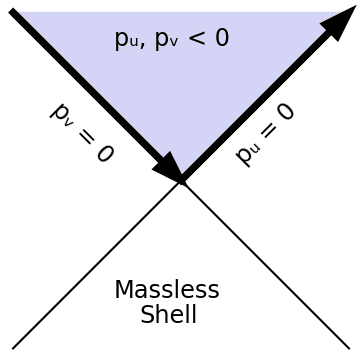
\includegraphics[scale=0.5]{massless_shell.png}
\caption{Massless shell is when $p_u$ = $p_v$ = 0}
\label{masslessshell}
\end{figure}

\begin{figure}[h]
\centering
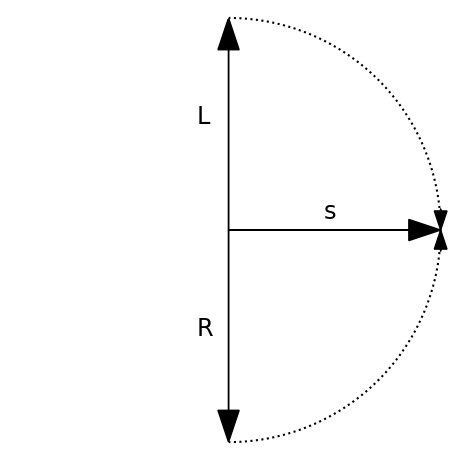
\includegraphics[scale=0.3]{contour.png}
\caption{Using contours with large radius we convert the $L$ integral that goes to $i\infty$, and the $R$ integral that goes to $-i\infty$, to integrals with $s$ going to real $\infty$.}
\label{fig:x cubed graph}
\end{figure}

We rewrite the integrals using a complex changes of variables, $s$ = $ip_uu$, and contour integrals.
The $L$ integral for real $p_u<0$ is
\begin{equation}
\begin{split}
  L(p_u) & = -\int_0^{i\infty} e^{-s}\left(\frac{ias}{-p_u}\right)^\frac{i\omega_k}{a} \left(\frac{i}{-p_u}\right)ds \\
  & = \frac{-i}{a} \left(\frac{a}{-p_u}\right)^{\frac{i\omega_k}{a} + 1} \int_0^\infty \left(is\right) ^ \frac{i\omega_k}{a} e^{-s} ds \\
  & = \frac{-i}{a} \left(\frac{a}{-p_u}\right)^{\frac{i\omega_k}{a} + 1} \Gamma\left(\frac{i\omega_k}{a} + 1\right) e^{-\frac{\pi \omega_k}{2a}} \\
  & = \frac{1}{2} \Gamma\left(\frac{i\omega_k}{a} + 1\right) e^{-\frac{\pi \omega_k}{2a}} B(p_u)\\
\end{split}
\end{equation}
where
\begin{equation}
B(p_u) = \frac{-2i}{a} \left(\frac{a}{-p_u}\right)^{\frac{i\omega_k}{a} + 1} 
\end{equation}
The change of $i\infty$ to $\infty$ is made by using a large radius contour which rotates the endpoint 90 degrees clockwise.  The term $e^{-s}$ goes to zero around the large radius circle.

The same calculation for $R$ is done using a counter-clockwise contour this time.
\begin{equation}
\begin{split}
  R(p_u) = \frac{1}{2}\Gamma\left(\frac{i\omega_k}{a} + 1\right) e^{-\frac{\pi \omega_k}{2a}} B(p_u)
\end{split}
\end{equation}

We get back to $f_k(u)$ and apply the normalization from equation (\ref{finalnorm})
\begin{equation}
\widehat{f_k}(p_u) = \frac{e^{\frac{\pi \omega_k}{2a}}}{\sqrt{2 \sinh \left({\frac{\pi\omega_k}{a}}\right)}}  ( L(p_u) + R(p_u) )
\end{equation}
So
\begin{equation}
\label{fourier}
\begin{split}
\widehat{f_k}(p_u) & = \frac{\Gamma\left(\frac{i\omega_k}{a} + 1\right)}{\sqrt{2 \sinh \left({\frac{\pi\omega_k}{a}}\right)}} B(p_u)\\
\widehat{g_k}(p_v) &= \frac{\Gamma\left(\frac{i\omega_k}{a} + 1\right)}{\sqrt{2 \sinh \left({\frac{\pi\omega_k}{a}}\right)}} B(p_v)
\end{split}
\end{equation}
\section{Interpretation}
The driving source $\rho$, with mixed absorption and emission thrusts $\alpha$ + $\beta$ = 1, contribute excitations to the scalar field $\phi$. Equations (\ref{ab}) and (\ref{fourier}) let us write down the expected change of energy
\begin{equation}  
  \label{number}
  \begin{split}
    \mathbb{E}[\Delta E] &= \frac{1}{4\pi} \int{|\rho(p)|^2 dp} \\
    &= \frac{\alpha}{4\pi} \int{\left|\widehat{f_k}(p_u)\right|^2 dp_u} + \frac{\beta}{4\pi}\int{\left|\widehat{g_k}(p_v)\right|^2dp_v} \\
    &= \frac{\left|\Gamma\left(\frac{i\omega_k}{a} + 1\right)\right|^2}{2 \sinh \left({\frac{\pi\omega_k}{a}}\right)} \frac{1}{4\pi} \int{{\left|B(p)\right|^2} dp} \\
    &=  \frac{\left|\Gamma\left(\frac{i\omega_k}{a} + 1\right)\right|^2}{2 \pi a \sinh \left({\frac{\pi\omega_k}{a}}\right)} \int{a/|p|^2 dp}\\  
&=I(\omega_k) P
  \end{split}
\end{equation}
where the integrals are on the positive energy massless shell with contributions from $p_u$ on the left piece and $p_v$ on the right piece.  We factored out $P = \int{a/|p|^2}$ with a remaining $p$ independent positive real coefficient $I(\omega_k)$.

Without being more careful we end up with inferred problems --- The integrals do not converge at zero, where $P$ explodes.  But this infinity cancels when we compare the spectral radiances to each other, $I(\omega_{k_1}) / I(\omega_{k_2})$.

The magnitude of our Gamma function has known asymptotics \cite[Eq.~5.11.9]{NIST:DLMF}
\begin{equation}
\left|\Gamma\left(\frac{i\omega_k}{a} + 1\right) \right|^2 \sim \left(\frac{2 \pi \omega_k} {a}\right) e^{-\frac{\pi\omega_k}{a}}
\end{equation}
Plugging this into equation (\ref{number}) we find the average energy of the mode, the $1+1$ dimensional Planck distribution function, and thus recover the Unruh's radiation spectrum from a thrust driven field.
\begin{equation}
\frac{1}{P} \mathbb{E}[\Delta E] = I(\omega_k) \sim \frac{\omega_k}{e^{\frac{2 \pi \omega_k}{a}}-1}
\end{equation}
Compare this to equation (\ref{radeq}) and references \cite{unruh} and \cite{Frodden}.

\begin{figure}[h]
\centering
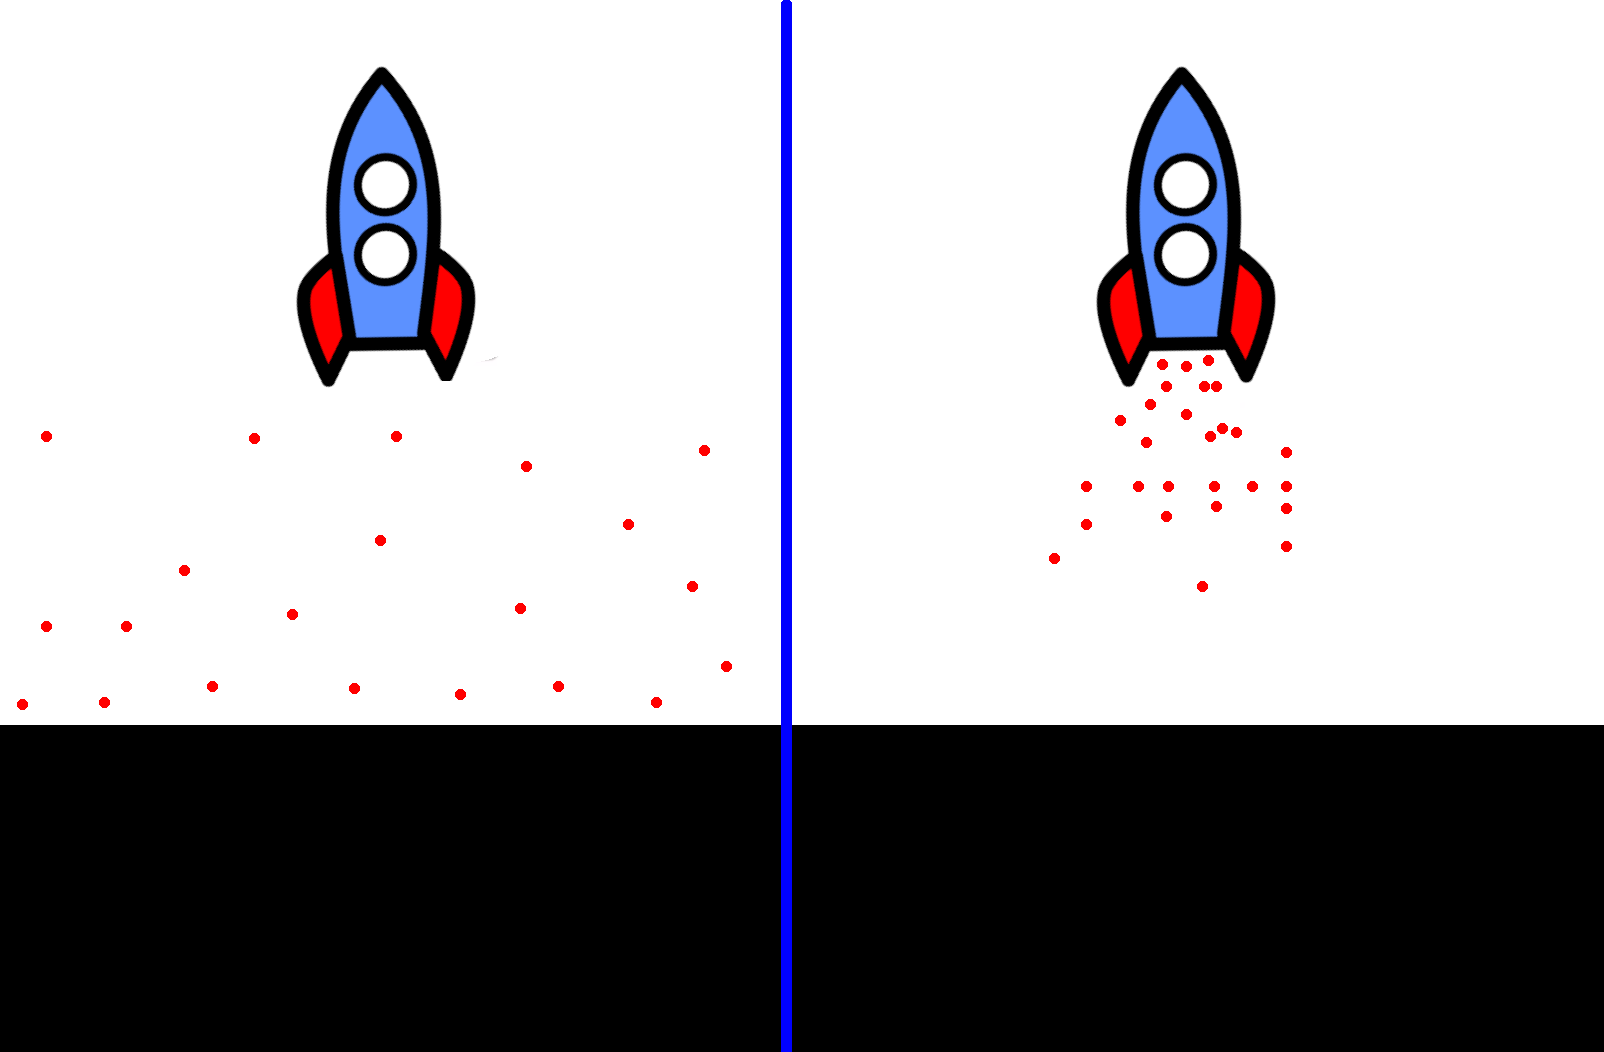
\includegraphics[scale=0.5]{rocket_inertial.png}
\caption{Unruh picture of an event horizon radiating in accelerating frame radiating on the left. Our picture of a rocket under inertial acceleration thrusting on the right.}
\label{rocket_inertial}
\end{figure}

\section{Other Types of Driving Sources}
TODO
\section{Ricci Scalar as a Driving Source}
TODO
\section{Fields with Interaction}
TODO

\section{Conclusion and Prediction}
If the thrust required to accelerate a detector is not explicitly accounted for, it manifests instead as an apparent thermal feature of the vacuum—Unruh radiation. However, as demonstrated in this paper, Unruh radiation can be directly explained as a consequence of thrust. This perspective leads to the prediction that neither Unruh radiation nor Hawking-Bekenstein radiation should appear independently of the thrust that drives the system.

\begin{figure}[h]
\centering
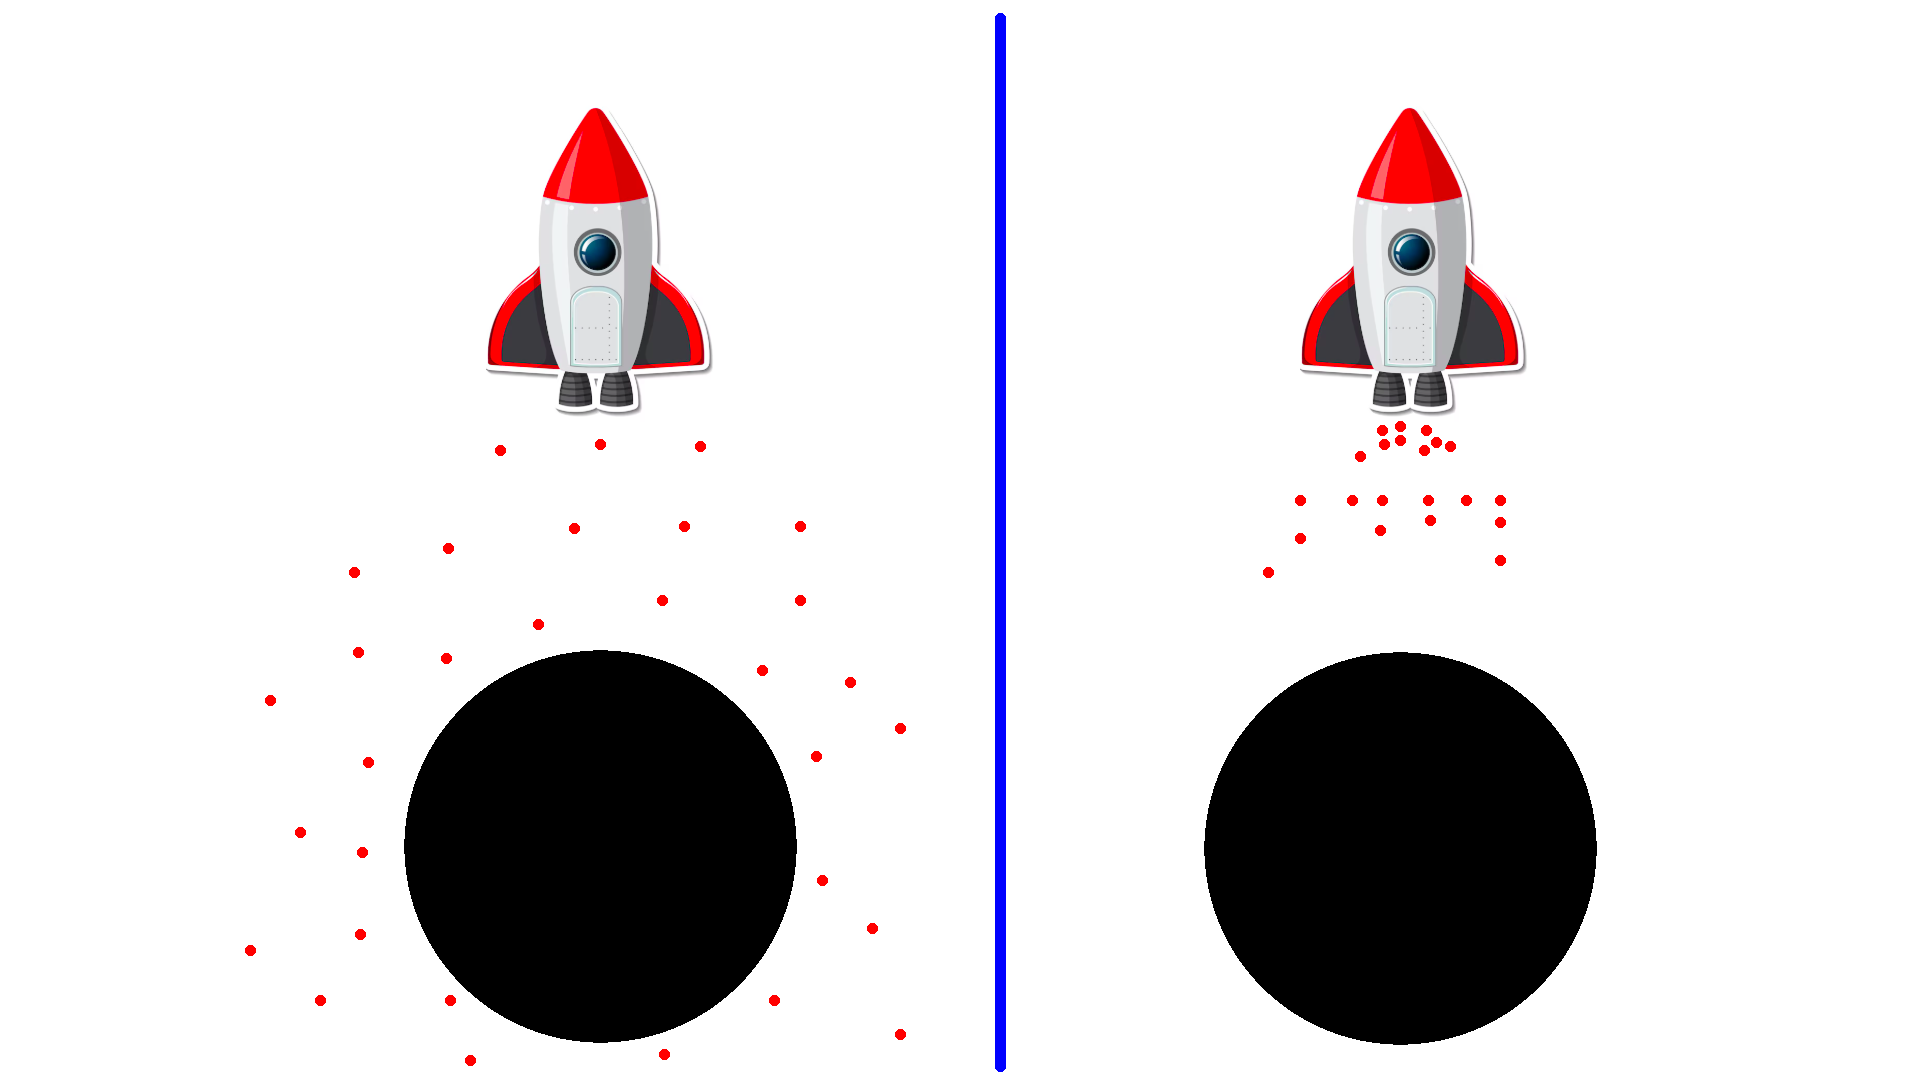
\includegraphics[scale=0.5]{rocket.png}
\caption{Hawking picture of black hole radiating on the left. Our picture of a rocket thrusting on the right.}
\label{rocket}
\end{figure}

\section{Acknowledgments}
Thanks to Ben Commeau and Daniel Justice for useful discussions.

\bibliographystyle{ieeetr}
\bibliography{bibliography}

\end{document}
